\documentclass{article}
%% This is the preamble
    \usepackage[utf8]{inputenc}
    \usepackage[dvipsnames,svgnames,x11names,table]{xcolor}
    %% To customize page margins, use geometry
    \usepackage{geometry}
    \geometry{top=1.5in,left=1in, right=1in, bottom = 1.5in}
    %% physics and math packages
    \usepackage{amsmath,derivative,siunitx}
    %% some helpful packages to make internal links in your document
    \usepackage{hyperref}
    %% to include pictures and plots
    \usepackage{graphicx}
    % extra packages for Quantum
    \usepackage{braket}
    \renewcommand{\doteq}{\,\dot{=}\,}


\title{Homework 4}
\author{Adrian deCola}
\date{March 16, 2023}


%% Now we begin the formal document
\begin{document}

\maketitle


\section*{Problem 9.28}
\verb+Problem+: Use the result (9.73) of Problem 9.26 to do the following: A naval gun shoots a shell at colatitude $\theta$ in a direction that is $ \aplha $ above the horizontal and due east, with muzzle speed $v_0$. (a) Ignoring the earth's rotation (and air resistance), find how long ($t$) the shell would be in the air and how far away ($R$) it would land. If $v_0= 500 \frac{m}{s}$ and $\alpha =$ 20°, what are $t$ and $R$? (b) A naval gunner spots an enemy ship due east at the range $R$ of part (a) and, forgetting about the Coriolis effect, aims his gun exactly as in part (a). Find by how far north or south, and in which direction, the shell will miss the target, in terms of $\Omega$, $v_0$, $\alpha$, $\theta$, and $g$. (It will also miss in the east—west direction but this is perhaps less critical.) If the incident occurs at latitude 50° north ($\theta$ = 40°), what is this distance? What if the latitude is 50° south? This problem is a serious issue in long-range gunnery: In a battle near the Falkland Islands in World War I, the British navy consistently missed German ships by many tens of yards because they apparently forgot that the Coriolis effect in the southern hemisphere is opposite to that in the north.


\begin{figure}[!h]
    \centering
    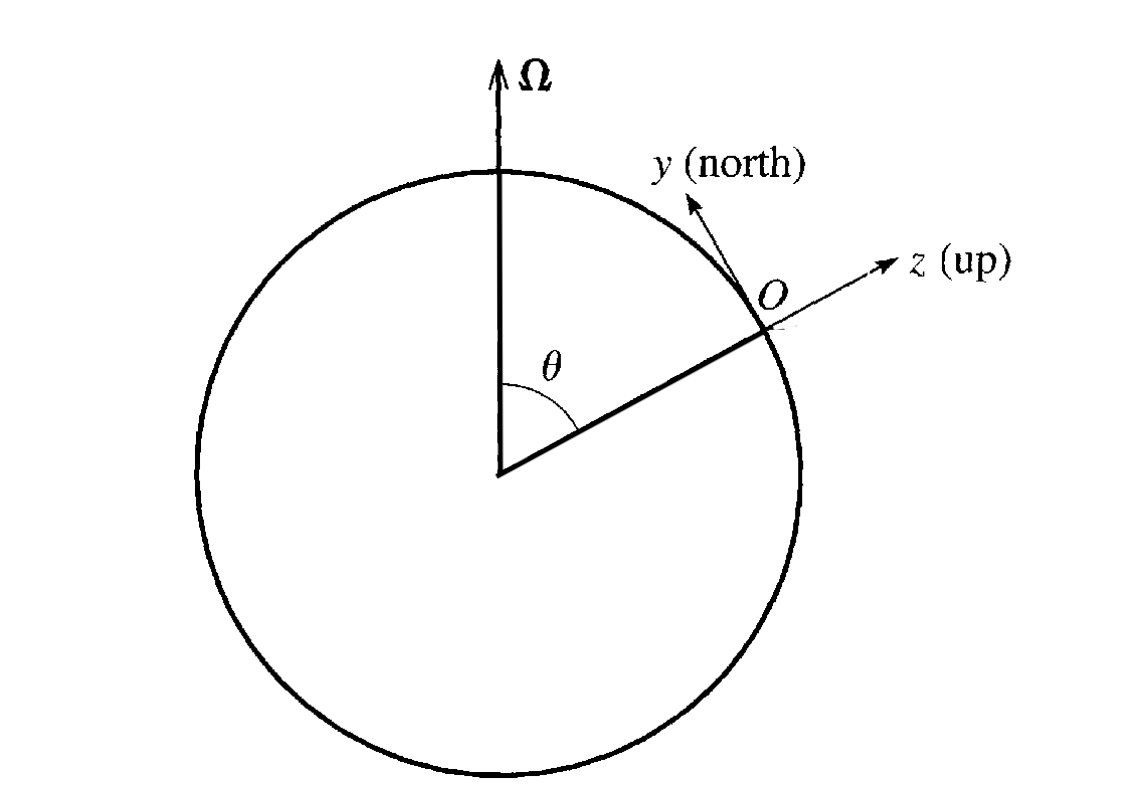
\includegraphics[width=.45\textwidth]{hw4_fig.png}
    \caption{An illustration of the coordinate axes we will use in this experiment where $x$ points east.}
\end{figure}

\begin{figure}[!h]
    \centering
    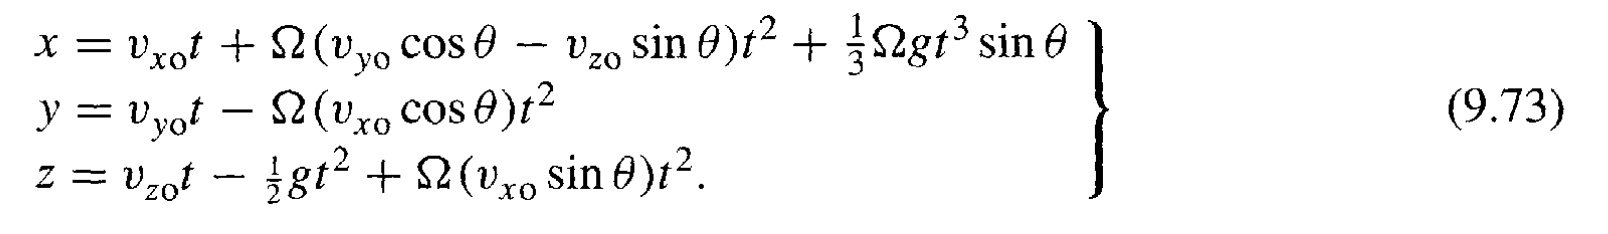
\includegraphics[width=.7\textwidth]{hw4_fig2.png}
    \caption{The results from Problem 9.26.}
\end{figure}

\hrule
         \ \ \ 
\subsection*{(a) Find the time the shell is in the air and how far away the shell lands ignoring the earth's rotations (and air resistance).}

We will use the usual kinematic equations to solve this problem as the acceleration is, to a great accuracy, constant. Since the shell is shot east with an angle above the horizon of $\alpha$: $v_{z,0} = v_0sin\alpha$, $v_{x,0} = v_0cos\alpha$, and $v_{y_0} = 0$. We know that the acceleration in the $z$ direction is $-g$. We also know that the naval gunner and enemy ship are at the same height: $\Delta z = 0$. Therefore, we can use the following kinematic equations to solve for the time the shell is in the air, ignoring the trivial solutions of $t=0$.
\begin{align*}
    \Delta &z = v_{z,0}t + \frac{1}{2}a_z t^2 \\
    &0 = v_0sin\alpha t + \frac{1}{2} (-g) t^2 \\
    &0 = v_0sin\alpha + \frac{1}{2} (-g) t \\
    &t = \frac{-v_0 sin\alpha }{-\frac{1}{2}g} \\
    &\boxed{t = \frac{2 v_0 sin\alpha }{g}} \\
\end{align*}

Since the shell is travelling eastward, we can use the same kinematics equations, but in the $x$ direction to get how far away the shell lands ($\Delta x = R$). There is no acceleration in the $x$ direction.  

\begin{align*}
    \Delta &x = v_{x,0}t + \frac{1}{2}a_x t^2 \\
    &R = v_0cos\alpha t  \\
    &R = v_0cos\alpha \frac{2 v_0 sin\alpha }{g}  \\
    &\boxed{R = \frac{2 v_0^2 sin\alpha cos\alpha}{g}}  \\
\end{align*}

Checking the units on both of these we get to correct dimensions. If $v_0= 500 \frac{m}{s}$ and $\alpha =$ 20°, we can solve for $t$ and $R$:
\begin{align*}
    &t = \frac{2 v_0 sin\alpha }{g} \\
    &t = \frac{2 (500) sin(20) }{9.807} \\
    &\boxed{t = 34.9 s} \\
\end{align*}
\begin{align*}
    &R = \frac{2 v_0^2 sin\alpha cos\alpha}{g}\\
    &R = \frac{2 (500)^2 sin(20) cos(20)}{9.807} \\
    &\boxed{R = 16.39  km}
\end{align*}

\subsection*{(b) Find by how far north or south, and in which direction, the shell will miss the target.}

For this section we will use the first order approximation results of the objects motion described in the equations 9.73. Figure 1 shows our coordinate system, where the shell is shot from the origin. As the shell is shot at the same initial velocity and angle: $v_{z,0} = v_0sin\alpha$, $v_{x,0} = v_0cos\alpha$, and $v_{y_0} = 0$. The Coriolis force has some component in the $z$ direction. We must therefore solve for the true time the shell is in the air by setting $z = 0 $ and ignoring the trivial solution of $t=0$. 

\begin{align*}
    z &= v_{z,0}t - \frac{1}{2}gt^2 + \Omega(v_{x,0}sin\theta)t^2 \\
    0 &= v_0sin\alphat - \frac{1}{2}gt^2 + \Omega v_0cos\alpha sin\theta t^2 \\
    0 &= v_0sin\alpha - \frac{1}{2}gt + \Omega v_0cos\alpha sin\theta t \\
    -v_0sin\alpha &=  (- \frac{1}{2}g + \Omega v_0cos\alpha sin\theta )t \\
    t &= \frac{-v_0sin\alpha}{- \frac{1}{2}g + \Omega v_0cos\alpha sin\theta}
\end{align*}

Using this result for the time the shell is in the air, we can now calculate $y$, the coordinate indicating the North-South displacement of the shell pointing North. 

\begin{align*}
    &y = v_{y,0}t - \Omega (v_{x,0}cos \theta ) t^2\\
    &y = - \Omega (v_{x,0}cos \theta ) t^2\\
    &y= -\Omega v_0cos\alpha cos\theta \left( \frac{-v_0sin\alpha}{- \frac{1}{2}g + \Omega v_0cos\alpha sin\theta}\right)^2 \\
    &y= -\Omega v_0cos\alpha cos\theta \frac{v_0^2 sin^2\alpha}{ \frac{1}{4}g^2 - g\Omega v_0cos\alpha sin\theta+ \Omega^2 v_0^2cos^2\alpha sin^2\theta} \\
    &\boxed{ y= \frac{-\Omega v_0^3 cos\alpha sin^2\alpha cos\theta}{\frac{1}{4}g^2 - g\Omega v_0cos\alpha sin\theta+ \Omega^2 v_0^2cos^2\alpha sin^2\theta} }
\end{align*}

Checking the units on this result we get the correct dimensions of length of meters. We also see that if we were not in a rotating frame, $\Omega=0$, there is no Coriolis force and no North-South movement as expected. We can solve for this value if the incident occurs at a latitude of 50° North or a colatitude of 40°($\theta$ = 40°). We know that the angular velocity of the Earth is $\Omega = 7.3 * 10^{-5} \frac{rad}{s}.$

\begin{align*}
    &y= \frac{-\Omega v_0^3 cos\alpha sin^2\alpha cos\theta}{\frac{1}{4}g^2 - g\Omega v_0cos\alpha sin\theta+ \Omega^2 v_0^2cos^2\alpha sin^2\theta}  \\
    &y = \frac{-(7.3 * 10^{-5}) (500)^3 cos(20) sin^2(20) cos(40)}{\frac{1}{4}(9.807)^2 - (9.807)(7.3 * 10^{-5}) (500)cos(20) sin(40)+ (7.3 * 10^{-5})^2 (500)^2 cos^2(20) sin^2(40)} \\
    &\boxed{y = -32.2 m}
\end{align*}
This means that at a latitude of 50° North, the shell strays 32.2 meters South of the target ship if the gunner does not take into account the Earth's rotation. This makes sense as we know the Coriolis force in the Northern Hemisphere pushes moving objects to the right, or (partially) South in this case. This is a large distance and it is clear how the Coriolis force must be taken into account for long-range gunnery. 

We can also solve for this value if the incident occurs at a latitude of 50° South ($\theta$ = 90° + 50° = 140°). 
\begin{align*}
    &y = \frac{-\Omega v_0^3 cos\alpha sin^2\alpha cos\theta}{\frac{1}{4}g^2 - g\Omega v_0cos\alpha sin\theta+ \Omega^2 v_0^2cos^2\alpha sin^2\theta}  \\
    &y = \frac{-(7.3 * 10^{-5}) (500)^3 cos(20) sin^2(20) cos(140)}{\frac{1}{4}(9.807)^2 - (9.807)(7.3 * 10^{-5}) (500)cos(20) sin(140)+ (7.3 * 10^{-5})^2 (500)^2 cos^2(20) sin^2(140)} \\
    &\boxed{y = 32.2 m}
\end{align*}

This means that at a latitude of 50° South, the shell strays 32.2 meters North of the target ship if the gunner does not take into account the Earth's rotation.  This makes sense as we know the Coriolis force in the Southern Hemisphere pushes moving objects to the left, or (partially) North in this case. These also both agree in magnitude with the British Navy missing German ship targets by tens of years in the Southern Hemisphere. 



\subsection*{Citation}
(1) Taylor, John R. Classical Mechanics. University Science Books, 2014. 


\end{document}